\usetikzlibrary{shapes, arrows, calc, positioning}

\tikzset{
    module/.style={
           rectangle,
           rounded corners,
           draw=black, very thick,
           minimum height=2em,
           inner sep=2pt,
           text centered,
           },
}


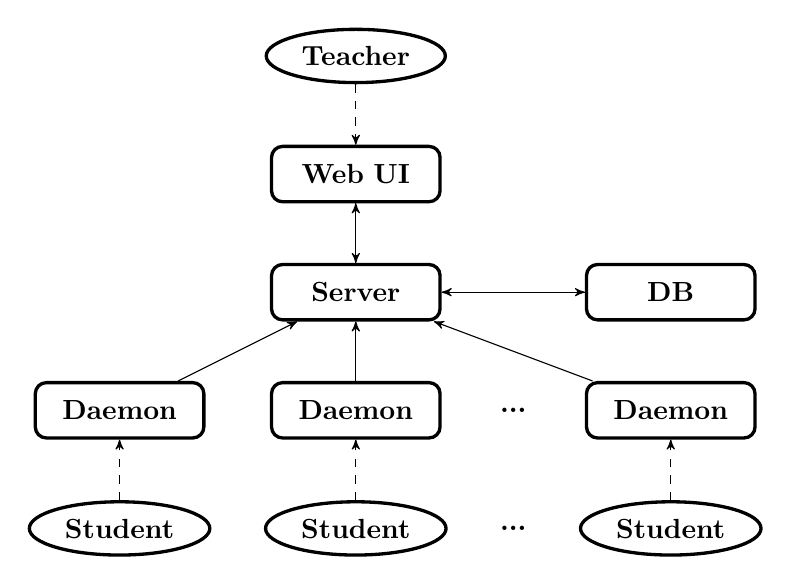
\begin{tikzpicture}[->,>=stealth']

 \node[ellipse, draw=black, very thick] (TEACHER)
 {%
  \textbf{Teacher}
 };

 \node[module,
  yshift=-0.5cm,
  text width=2cm,
  below of=TEACHER] (UI)
 {%
  \textbf{Web UI}
 };

 \node[module,
  text width=2cm,
  yshift=-0.5cm,
  below of=UI] (SERVER)
 {%
  \textbf{Server}\\
 };

 \node[module,
  below of=SERVER,
  yshift=-0.5cm,
  xshift=-3cm,
  anchor=center,
  text width=2cm] (DAEMON_1)
 {%
  \textbf{Daemon}
 };

 \node[module,
  right of=DAEMON_1,
  xshift=2cm,
  text width=2cm] (DAEMON_2)
 {%
  \textbf{Daemon}
 };

 \node[module,
  right of=DAEMON_2,
  xshift=1cm,
  draw=none,
  text width=1cm] (HIDDEN_DAEMONS)
 {%
  \textbf{...}
 };

  \node[module,
  right of=HIDDEN_DAEMONS,
  xshift=1cm,
  text width=2cm] (DAEMON_3)
 {%
  \textbf{Daemon}
 };

 \node[module,
  right of=SERVER,
  xshift=3cm,
  text width=2cm] (DB)
 {%
  \textbf{DB}
 };

 \node[ellipse, draw=black, very thick,
       below of=DAEMON_1,
       yshift=-0.5cm, ] (STUDENT_1)
 {%
  \textbf{Student}
 };

  \node[ellipse, draw=black, very thick,
       below of=DAEMON_2,
       yshift=-0.5cm, ] (STUDENT_2)
 {%
  \textbf{Student}
 };

  \node[ellipse,
       below of=HIDDEN_DAEMONS,
       yshift=-0.5cm, ] (HIDDNE_STUDENT)
 {%
  \textbf{...}
 };

  \node[ellipse, draw=black, very thick,
       below of=DAEMON_3,
       yshift=-0.5cm, ] (STUDENT_3)
 {%
  \textbf{Student}
 };

 \path (DAEMON_1) edge (SERVER);
 \path (DAEMON_2) edge (SERVER);
 \path (DAEMON_3) edge (SERVER);

 \path (SERVER) edge (DB);
 \path (DB) edge (SERVER);

 \path (SERVER) edge (UI);
 \path (UI) edge (SERVER);

 \path (TEACHER) edge[dashed] (UI);

 \path (STUDENT_1) edge[dashed] (DAEMON_1);
 \path (STUDENT_2) edge[dashed] (DAEMON_2);
 \path (STUDENT_3) edge[dashed] (DAEMON_3);

\end{tikzpicture}